\documentclass{beamer}
\usepackage{xcolor}
%\usepackage{fontspec}
%\setmainfont{Georgia}
%\usepackage[T1]{fontenc}
\usepackage{winfonts}
\usepackage[backend=bibtex]{biblatex}
\renewcommand{\sfdefault}{georgia}

\bibliography{report}

%%%%%%%%%%%%%%
% Soton colourscheme

%primary palette:           RED    GREEN  BLUE
\definecolor{sotonblu}{rgb}{.00392 .26275 .34902} % soton blue
\definecolor{sotongrn}{rgb}{.00000 .44706 .45882} % soton green
\definecolor{sotoncya}{rgb}{.03922 .58824 .66275} % soton cyan
\definecolor{sotongry}{rgb}{.19608 .23922 .26275} % soton grey
\definecolor{sotonbei}{rgb}{.59216 .61961 .27059} % soton beige
\definecolor{sotonmet}{rgb}{.73333 .73333 .73333} % soton metal

%some secondary colors:
\definecolor{sotonyel}{rgb}{.99999 .70196 .00000} % soton yellow
\definecolor{sotonora}{rgb}{.99608 .24314 .07843} % soton orange
\definecolor{sotonred}{rgb}{.94118 .05882 .17255} % soton red
\definecolor{sotonrus}{rgb}{.67059 .07059 .06275} % soton russet
\definecolor{sotonbrn}{rgb}{.54118 .25490 .16863} % soton brown
\definecolor{sotonpnk}{rgb}{.88627 .41176 .62353} % soton pink
\definecolor{sotonppl}{rgb}{.32549 .12157 .26667} % soton purple


\setbeamertemplate{background canvas}[vertical shading][top=sotonblu,bottom=sotoncya]
\setbeamercolor{background canvas}{bg=}
\setbeamercolor{button border}{bg=sotonblu, fg=sotonblu}
\setbeamercolor{button}{bg=sotonblu, fg=DarkRed}

\setbeamercolor{frametitle}{fg=sotonyel}
\setbeamercolor{alerted text}{fg=sotonyel}
\setbeamercolor{normal text}{fg=white}
\setbeamercolor{titlelike}{fg=sotonyel}
\setbeamercolor{author}{fg=white}
\setbeamercolor{date}{fg=white}
\setbeamercolor{item}{fg=white}

%%%%%%%%%%%%%%%%%%%%

\title{Identification of the Curie Temperature Distribution from
Temperature Dependent Magnetisation Data}
\author{Jonathon Waters\inst{1}, Hans Fangohr\inst{1}, Denis Kramer\inst{1}, Andreas Berger\inst{2} and Ondrej Hovorka\inst{1}}
\institute{
	\inst{1}
	Engineering and the Environment,\\
	University of Southampton,\\
	UK\\
	\inst{2}
	Somewhere
}
\date{}

\begin{document}
\frame{\titlepage 

\includegraphics[height=1cm]{Images/sponsor-wo}\hfill
\includegraphics[height=1cm]{Images/uos_grey_large}}

\setbeamertemplate{headline}{
	\vskip25pt % horizontal line
	\vskip-21pt\hspace{2pt}\hfill
\includegraphics[height=7mm]{Images/sponsor-wo}\hspace{3.5mm}
\includegraphics[height=7mm]{Images/uos_grey_large}\hspace{3.5mm} % logo on the right
}

\setbeamertemplate{footline}{
	\vskip-8pt % horizontal line
	\hspace{12cm} \insertframenumber/\inserttotalframenumber
	\vskip4pt
}

\begin{frame}
	\frametitle{Introduction}
	\begin{columns}
		\column{6cm}
		In HAMR\footnotemark[1]:
		\begin{itemize}
			\item{$T_C$ distribution affects the noise performance.}
		\end{itemize} \vspace{4mm}
		
		\begin{center}
		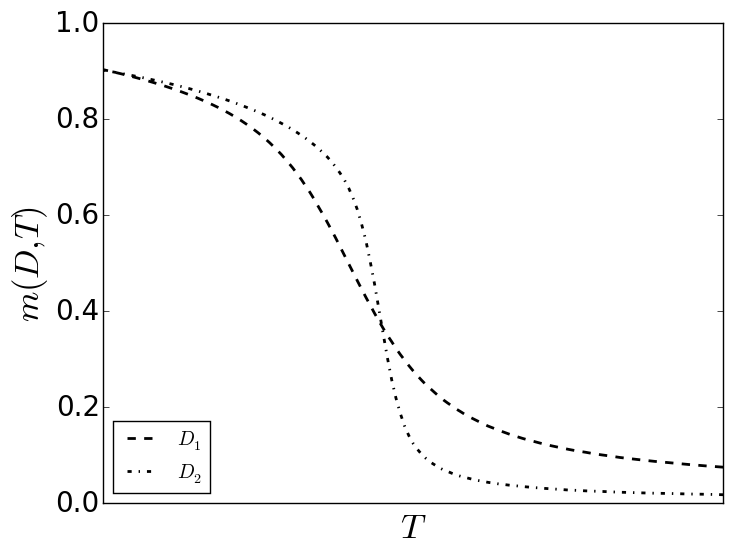
\includegraphics[width=4cm]{Images/Ds_noinset} \\ \vspace{3mm}
		\end{center}
		
		\column{6cm}
		In Magnetic Hyperthermia\footnotemark[2]:
		\begin{itemize}
		\item{Low $T_C$ reduces tissue damage.}
		\end{itemize} \vspace{1mm}
		
		\begin{center}
		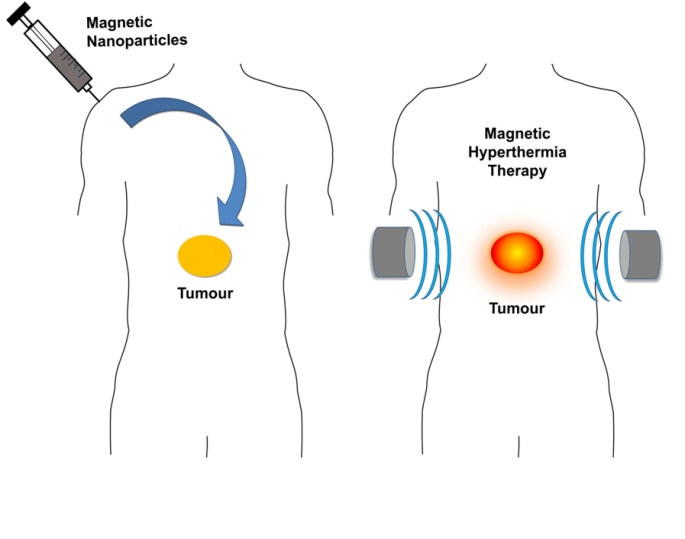
\includegraphics[width=4cm]{Images/person} \\
		\tiny \^{A}ngela Andrade, Roberta Ferreira, Jos\'{e} Fabris and Rosana Domingues (2011). Coating Nanomagnetic Particles for Biomedical Applications
		\end{center}
	\end{columns}
	\footnotetext[1]{\tiny \fullcite{weller2014hamr}}
	\footnotetext[2]{\tiny \fullcite{apostolova2009possible}}
\end{frame}

\begin{frame}
	\frametitle{Finite Sized $T_C$}
	\begin{columns}
		\column{6cm}
		\begin{center}
		Correlation length $\propto |T-T_C^b|^{-\nu}$ \\ \vspace{3mm}
		Grain size, $D \propto |T_C(D)-T_C^b|^{-\nu}$ \\ \vspace{3mm}
		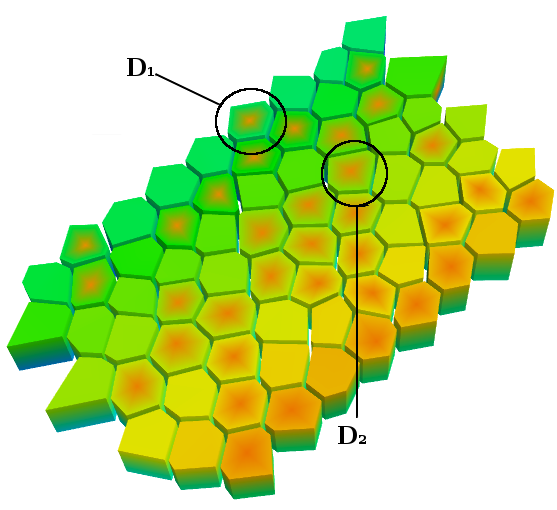
\includegraphics[width=5cm]{Images/grains2}
		\end{center}
		\column{6cm}
		\begin{center}
		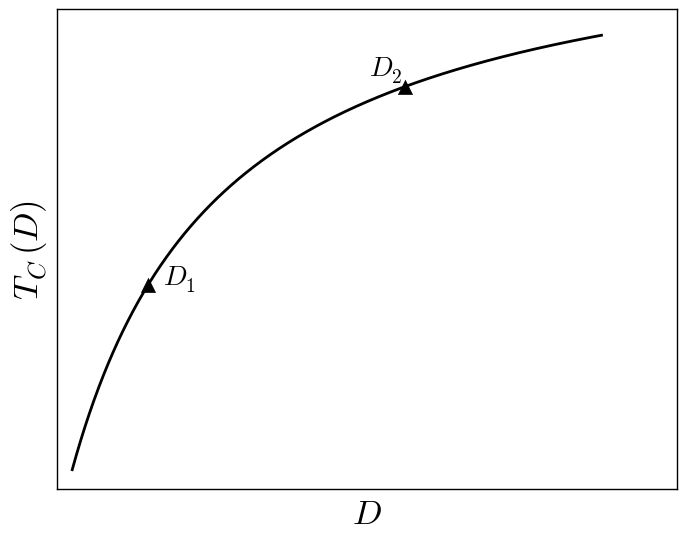
\includegraphics[width=5cm]{Images/TcD}
		\end{center} \vspace{4mm}
		$$
		f_D(D) \Longrightarrow f_{T_C}(T_C)
		$$
	\end{columns}
\end{frame}

\begin{frame}
	\frametitle{Previous Methods}
	2 Types:
	\vspace{4mm}
	\begin{itemize}
		\item{Explicit measurement of individual grains.\footnotemark[3]}
		\vspace{4mm}
		\item{Implicit calculation using global measurements.\footnotemark[4]}
		\begin{itemize}
			\item{Single measurement with magnetometer}
			\item{Integral measure}
			\item{Uses bulk relations}
		\end{itemize}
	\end{itemize}	
	\footnotetext[3]{\tiny \fullcite{pisana2015curie}}
	\footnotetext[4]{\tiny \fullcite{berger2002critical}}
\end{frame}

\begin{frame}
	\frametitle{Objectives}
	\begin{itemize}
		\item{Develop a method to identify the $T_C$ distribution which incorporates the finite size effects of the individual grains.\newline}
		\item{Test this method against benchmark data in order to verify it's effectiveness for different distributions.\newline}
	\end{itemize}
\end{frame}

\begin{frame}
	\frametitle{Our Method}
	\begin{columns}
	\column{8cm}
	Aggregate Magnetisation:
	$$
	M(T) = M_0\int_0^\infty D^{d} m(D,T) f_D(D) dD
	$$
	Scaling Ansatz:
	$$
	m(D,T) \propto D^{-\beta/\nu} \mu \left(D^{1/\nu}\frac{T-T_C^b}{T_C^b}\right)
	$$
	Change of Variables:
	$$
	D = d_0\left(\frac{t}{T_C^b}\right)^{-\nu}\quad	t \equiv T_C^b - T_C(D)
	$$
	Final Result:
	$$
	M(T) = M_0^*\int_0^{T_C^b} t^{-d\nu +\beta} \mu\left(d_0^{\frac{1}{\nu}}\frac{T-T_C^b}{t}\right) f_t(t) dt
	$$
	\column{4cm}
	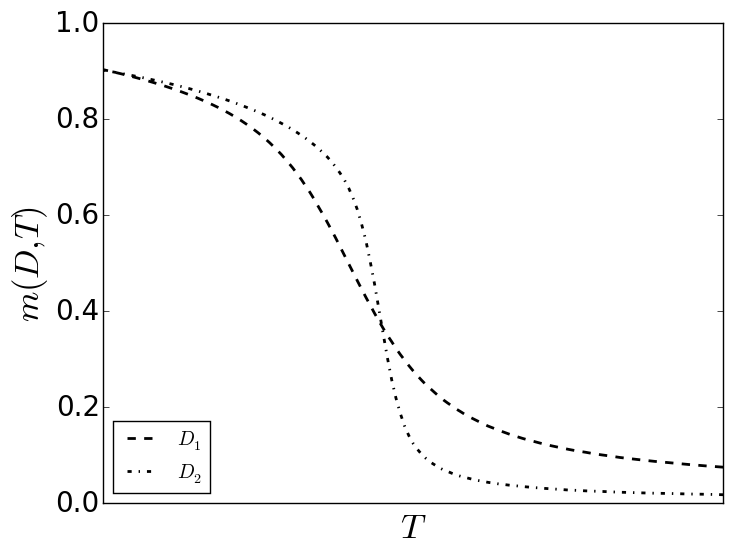
\includegraphics[width=4cm]{Images/Ds_noinset}
	
	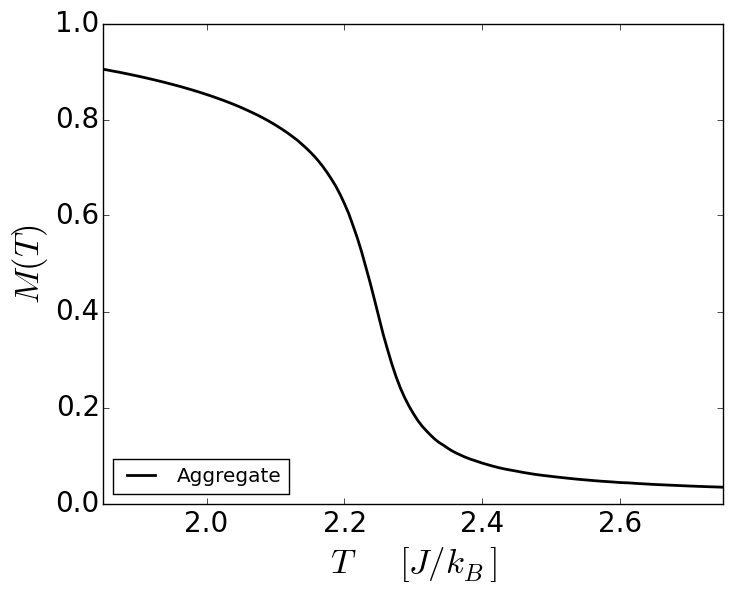
\includegraphics[width=4cm]{Images/Aggregate}
	\end{columns}
\end{frame}

\begin{frame}
	\frametitle{Finding $f_t$}
	$$
	M(T) = M_0^*\int_0^{T_C^b} t^{-d\nu +\beta} \mu\left(d_0^{\frac{1}{\nu}}\frac{T-T_C^b}{t}\right) f_t(t) dt
	$$
	
	\begin{itemize}
		\item{$M(T)$: To be fitted}
		\item{$d$, $\nu$, $\beta$, $\mu$: Known information about the material}
		\item{$d_0$, $T_C^b$: May be known, otherwise taken from fit}
		\item{$M_0^*$, $f_t$ [ $\bar{t}$, $\sigma_t$ ]: Taken from the fit}
	\end{itemize}
	
	\begin{center}
	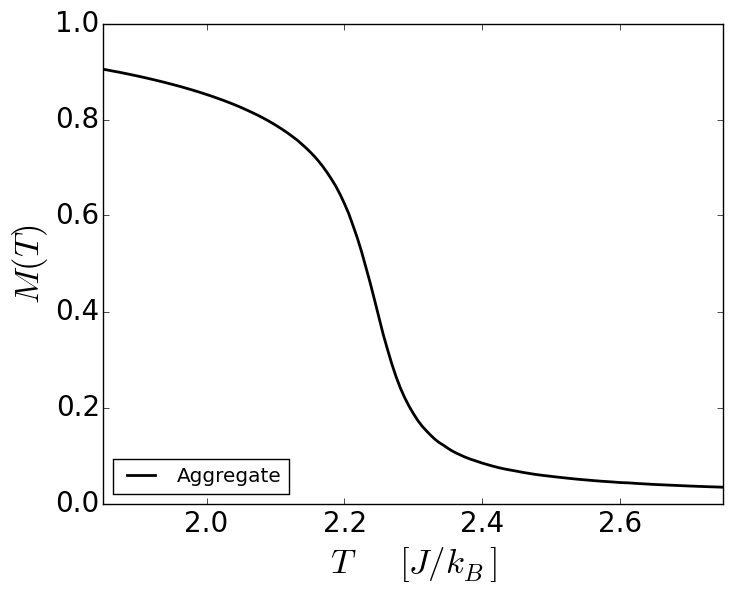
\includegraphics[width=5cm]{Images/Aggregate} \hspace{3mm}
	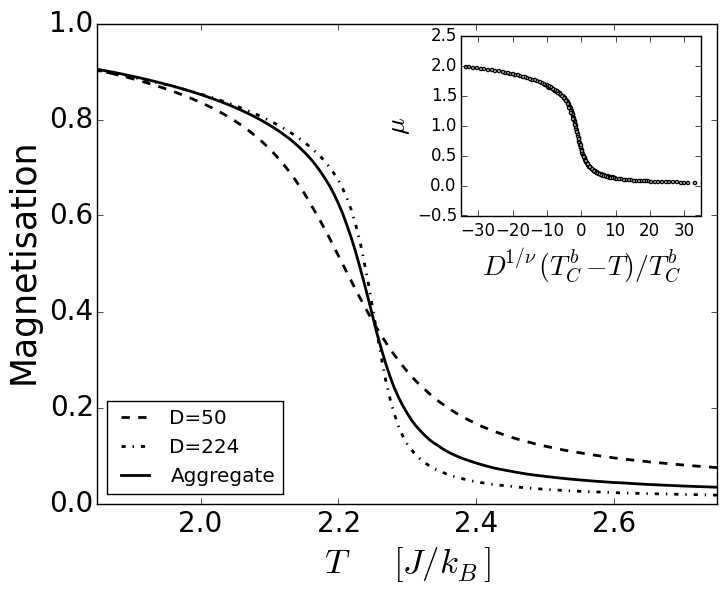
\includegraphics[width=5cm]{Images/Ds}
	
	\end{center}
\end{frame}

\begin{frame}
	\frametitle{Test Case: 2D Ising Model}
	\begin{columns}
	\column{7cm}
		Used 2D Ising model as a benchmark:
		\begin{itemize}
			\item{Easilly simulated}
			\item{Analytical results for $\beta$, $\nu$, $T_C^b$...}
		\end{itemize} \vspace{4mm}
		
		Tested against different $f_D$:
		\begin{itemize}
			\item{All mean $\bar{D}=100$}
			\item{Standard deviation $\sigma_D=10, 20, 30 ,40$}
		\end{itemize}
	\column{5cm}
		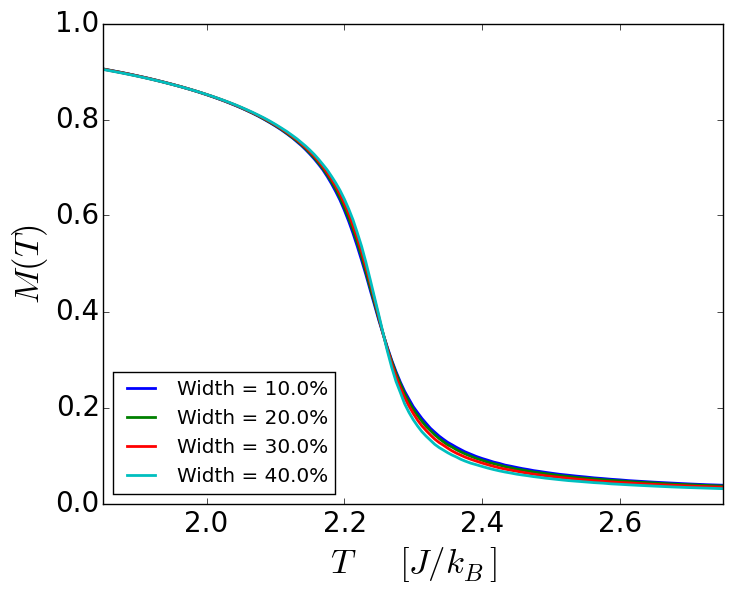
\includegraphics[width=4.5cm]{Images/distros}
		
		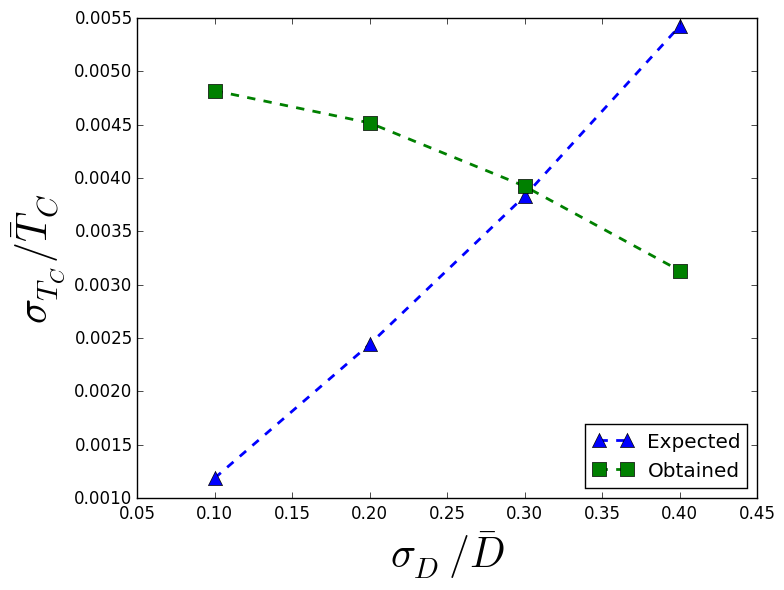
\includegraphics[width=4.5cm]{Images/unconst}
	\end{columns}
\end{frame}

\begin{frame}
	\frametitle{Test Case: 2D Ising Model}
	\begin{columns}
	\column{7cm}
		Introduce constraint from:
		$$
		D = d_0\left(\frac{t}{T_C^b}\right)^{-\nu}
		$$
		
		$$\Rightarrow \sigma_t^2 = \bar{t}^2\left(\left(1 + \frac{\sigma_D^2}{\bar{D}^2}\right)^{1/\nu^2}-1\right)
		$$
		
		\begin{center}
		Works much better!
		\end{center}
	\column{5cm}
		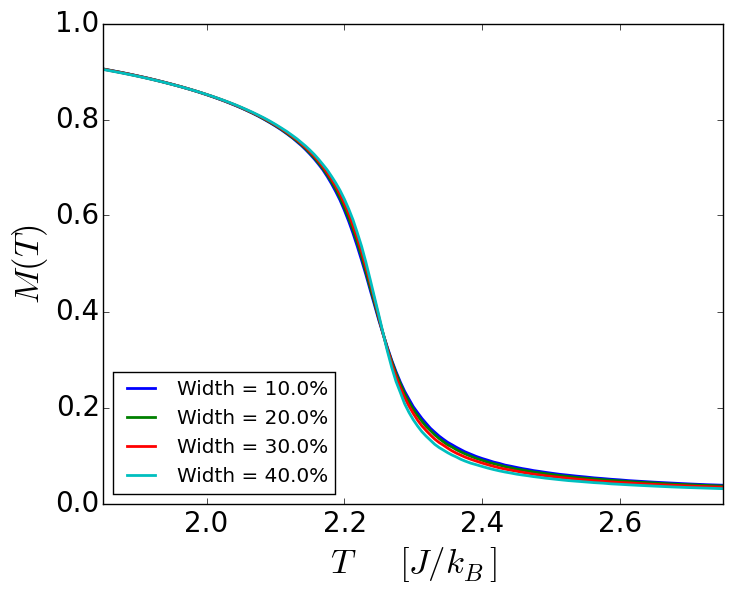
\includegraphics[width=4.5cm]{Images/distros}
		
		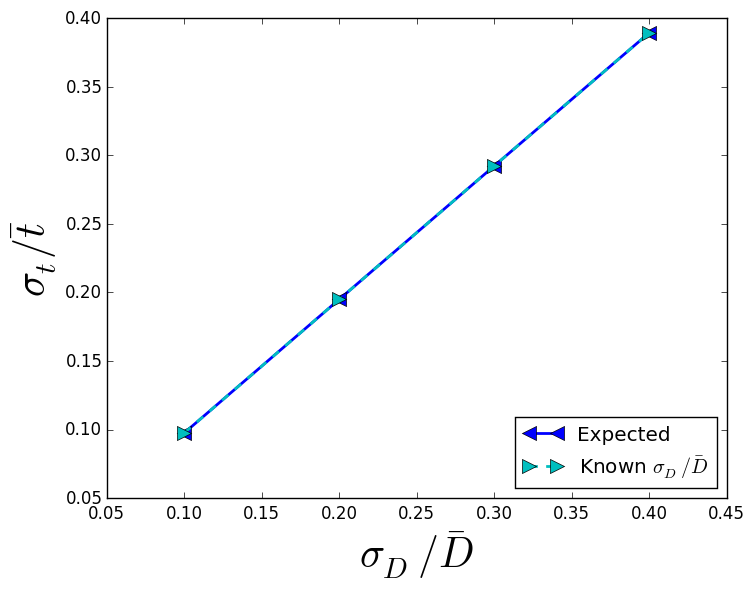
\includegraphics[width=4.5cm]{Images/constr}
	\end{columns}
\end{frame}

\begin{frame}
	\frametitle{Conclusions}
	\begin{itemize}
		\item{Presented a universal method to find size dependent $T_C$ distribution.}
		\item{Based upon fitting ensemble magnetisation:}
		$$
		M(T) = M_0^*\int_0^{T_C^b} t^{-d\nu +\beta} \mu\left(d_0^{\frac{1}{\nu}}\frac{T-T_C^b}{t}\right) f_t(t) dt
		$$
		\item{Successfully tested against different size distributions $f_D$, given certain constraints.}
	\end{itemize}
\end{frame}

\begin{frame}
	\frametitle{Acknowledgements}
	In the completion of this work, we acknowledge financial support from the EPSRC Centre for Doctoral Training grant EP/L006766/1. \newline
	
	We also acknowledge the use of the IRIDIS High Performance Computing Facility, and associated support services at the University of
Southampton. \newline

	Contact: J.M.Waters@soton.ac.uk
\end{frame}
\end{document}